\documentclass[12pt, a4paper]{article}
\usepackage[utf8]{inputenc}
\usepackage{graphicx}
\usepackage{gensymb}
\usepackage{amsmath}
\usepackage{float}
\usepackage{subcaption}
\usepackage{caption}


\title{ODE IVP}
\author{Miha Pompe}
\date{November 2021}

\begin{document}
\begin{titlepage}
	\centering
 	
\includegraphics[width=0.45\textwidth]{logo_fmf_uni-lj_sl_veliki.png}\par\vspace{1cm}

	\vspace{1cm}

	\vspace{1.5cm}
	{\huge\bfseries Initial value problem for first order ordinary differential equations\par}
	\vspace{2cm}
	{\Large Miha Pompe 28191072\par}
	\vfill

	\vfill

% Bottom of the page
	{\large November 2021\par}
\end{titlepage}
% \maketitle
\thispagestyle{empty}
\clearpage
\pagenumbering{arabic}
\newpage


\section{Introduction}
The simplest physical processes can be described using ordinary differential equations that relate a given variable with it's change in time. In this report we will use an example of temperature change in an apartment, which is surrounded by walls with a given thermal conductivity and a set outside temperature ($T_{out}$). The equation for this examples is:

\begin{equation}
  \frac{dT}{dt} = -k(T - T_{out})
\end{equation}
which can be solved analytically
\begin{equation}
  T(t) = T_{out} + e^{-kt}(T(0) - T_{out})
\end{equation}

In this report we will be studying numerical methods for solving the first equation. Most methods use the initial differential equation to calculate the derivative in a certain point and use it to calculate the next point, meaning points are generated sequentially.

\section{Method analysis}
Methods used to analyse out initial value problem are: Euler, Heun, midpoint, second-order Runge-Kutta (RK2), fourth-order Runge-Kutta (RK4), fourth-order Runge-Kutta with error estimate (RK45), Runge-Kutta-Fehlberg (RKF), Adams-Bashforth-Moulton fourth-order predictor-corrector (PC4) and built in function Odeint ({\sc scipy.integrate.odeint}). If not stated otherwise the paramaters and initial values are k = 0.1, h = 0.1, $T_out = 5^{\circ}C$.

Using the methods above we can solve our problem and see the solutions in Figure 1, for $T(0) = 21^{\circ}C$ and $T(0) = -15^{\circ}C$. As expected the result is a moved and scaled exponential function. To determine the accuracy of the method we will use the analytical solution. The most accurate method is RKF, achieving error up to $10^-6 ^{\circ}C$, when selecting $10^-3 ^{\circ}C$ tolerance threshold. All other methods achieve similar accuracy. I presume the peak is the result of our numerical solution crossing the analytical function. The absolute error tends to decrease with time, as we are quickly approaching the asymptote. This observation does not hold for longer times. The last two graphs of Figure 1 show the impact of parameter $k$, which goes from the value $0.05$ to $1$ (yellow to violet). The lower the parameter, the slower we reach the equilibrium. Therefore we can assume $k$ is proportional to thermal conductivity. The method RKF was used to calculate these solutions, as it is able to achieve the best accuracy.

\begin{figure}[hbtp]
  \begin{center}
  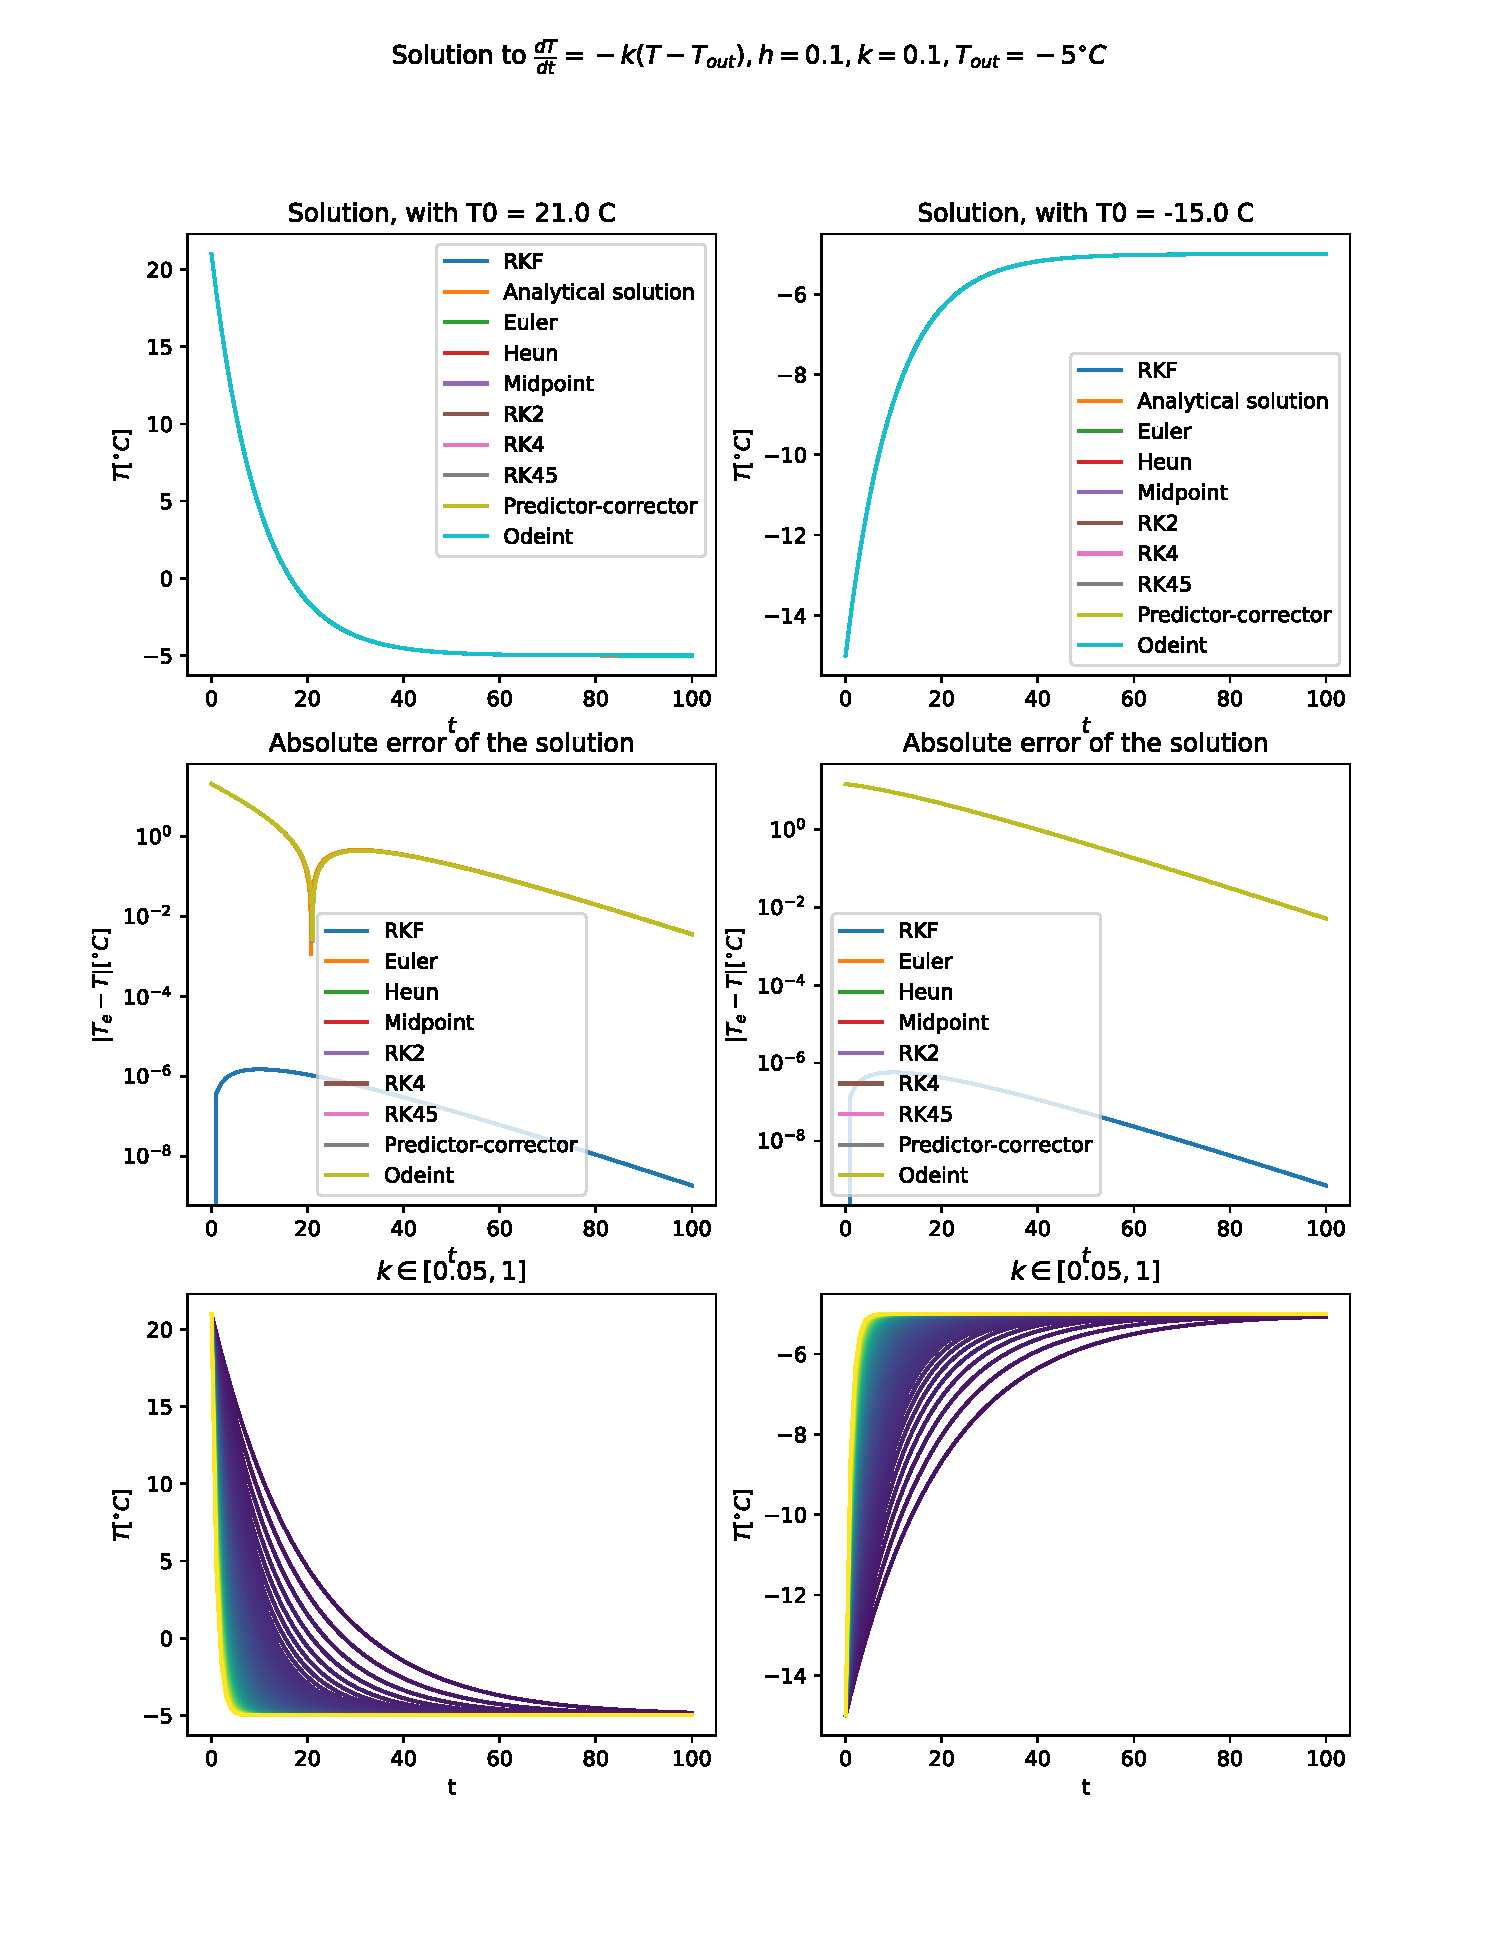
\includegraphics[width=13cm]{graphs/solution.pdf}
  \end{center}
  \vspace*{-7mm}
  \caption{Solution analysis for the room temperature problem.}
\end{figure}

Furthermore we can analyse the methods by changing other parameters. The most important factor for almost all of the methods is the step size $h$, which is defined as $h = t[i+1] - t[i]$. Looking at Figure 1a we notice linear patterns (in the log-log scale). The worst performing is Euler method where error increases linearly with step size. Following are Heun, midpoint and RK2 that all increase quadratically. The best performing are RK4, RK45 and predictor-corrector methods where error increases with $h^4$. On the lower end at around $h = 10^{-2}$ we reach a plateau, corresponding to the numerical limit. The global error of Odeint method does not appear to change with $h$. Similar analysis was performed in Figure 2b, but here we also look at time dependence. We observe that the error increases with time and step size.

\begin{center}
  \begin{tabular}{ c c c }
   Method & Global error & Computation time \\
   \hline 
   Euler & $\mathcal{O}(h)$ & $\mathcal{O}(\frac{1}{h})$ \\  
   Heun & $\mathcal{O}(h^2)$ & $\mathcal{O}(\frac{1}{h})$ \\  
   Midpoint & $\mathcal{O}(h^2)$ & $\mathcal{O}(\frac{1}{h})$ \\  
   RK2 & $\mathcal{O}(h^2)$ & $\mathcal{O}(\frac{1}{h})$ \\  
   RK4 & $\mathcal{O}(h^4)$ & $\mathcal{O}(\frac{1}{h})$ \\  
   RK45 & $\mathcal{O}(h^4)$ & $\mathcal{O}(\frac{1}{h})$ \\  
   Predictor-corrector & $\mathcal{O}(h^4)$ & $\mathcal{O}(\frac{1}{h})$
  \end{tabular}
  \end{center}

The second important factor is computation time and it's dependence on step size. From Figure 2c we can conclude that computation time rises with smaller step sizes linearly. Step size is inversely proportional to the number of elements in a certain time frame, therefore the time complexity is $\mathcal{O}(N) = \mathcal{O}(\frac{1}{h})$. This relation comes from the use of one for loop. For a given step size we can see differences in computation times, which come from the time needed to perform one step of the algorithm. Therefore we can order the methods by speed in the following way going from fastest to slowest: Euler, RK2, Heun, midpoint, predictor-corrector, RK4 and RK45. Computation time of Odeint method rises linearly with lower step sizes, but reaches a plateau at higher $h$. In the limit $h \rightarrow 0$ this method would be the fastest. 

\begin{figure}[hbtp]
  \begin{subfigure}{0.5\textwidth}
  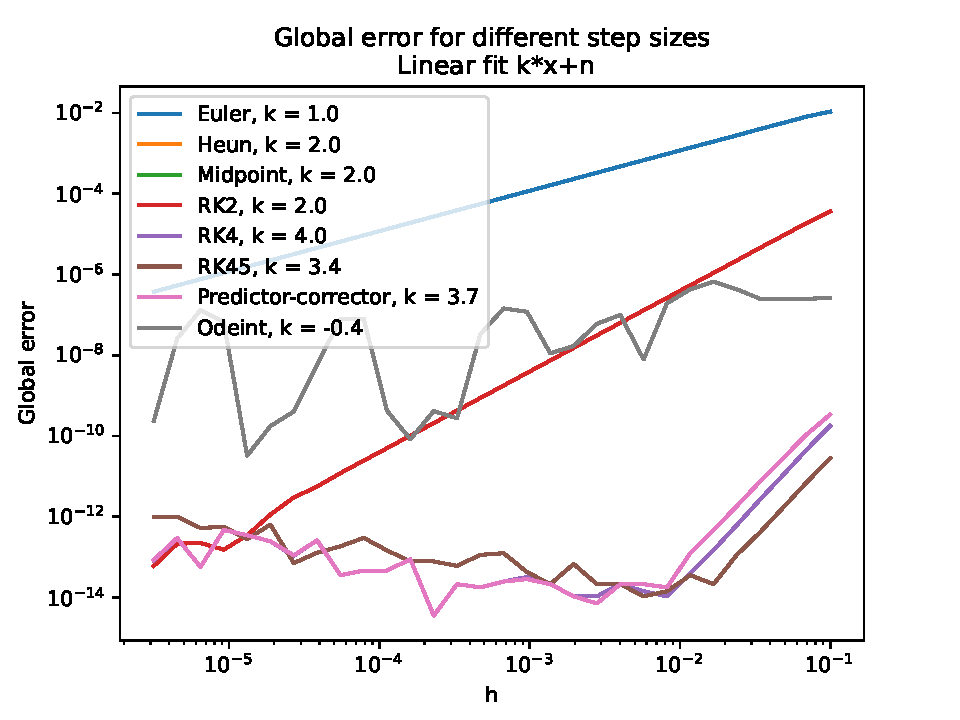
\includegraphics[width=\linewidth]{graphs/error_h.pdf}
  \caption{Global error for different step sizes.} \label{fig:a}
  \end{subfigure}
  \hspace*{\fill}
  \begin{subfigure}{0.5\textwidth}
  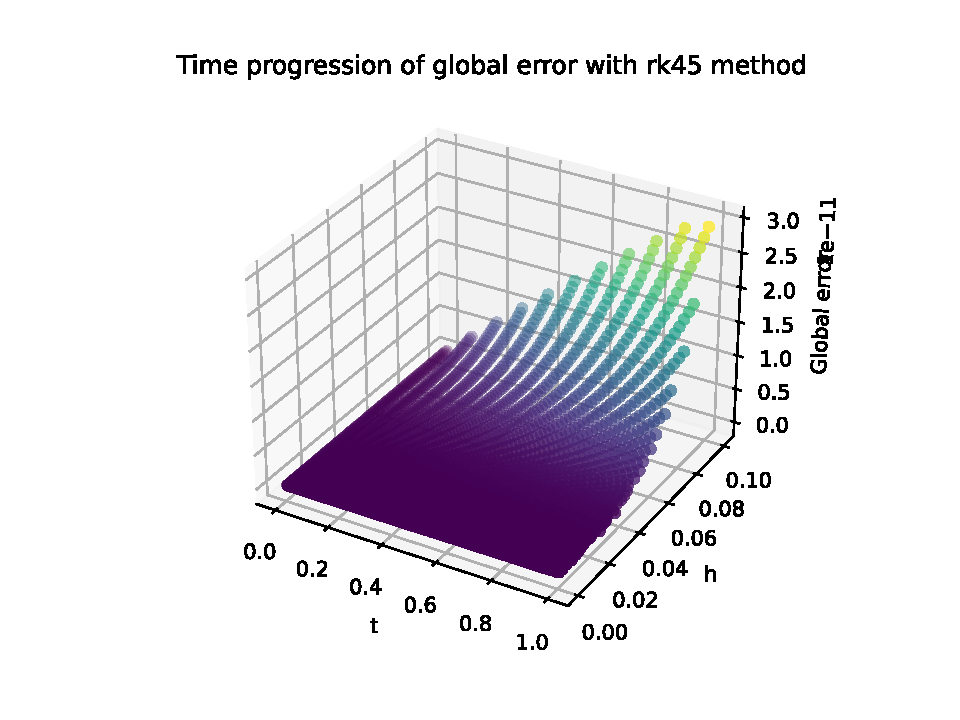
\includegraphics[width=\linewidth]{graphs/error_3D.pdf}
  \caption{Global error as a function of $h$ and $t$, color is proportional to the error.} \label{fig:b}
  \end{subfigure}
  \medskip
  \begin{subfigure}{0.5\textwidth}
  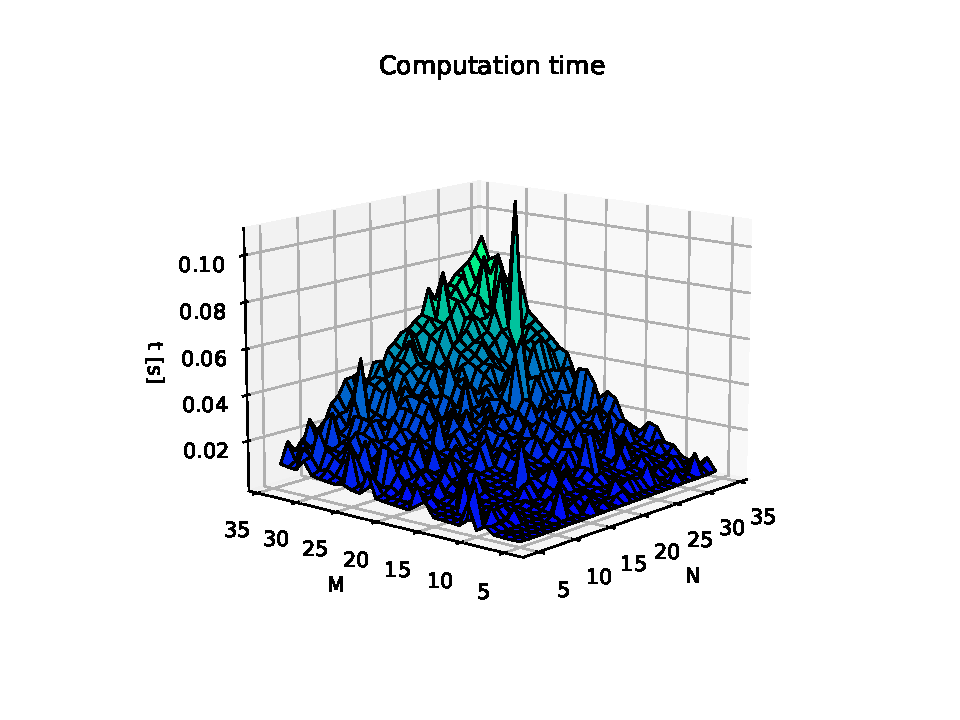
\includegraphics[width=\linewidth]{graphs/time.pdf}
  \caption{Computation time for different step sizes.} \label{fig:c}
  \end{subfigure}
  \hspace*{\fill}
  \begin{subfigure}{0.5\textwidth}
  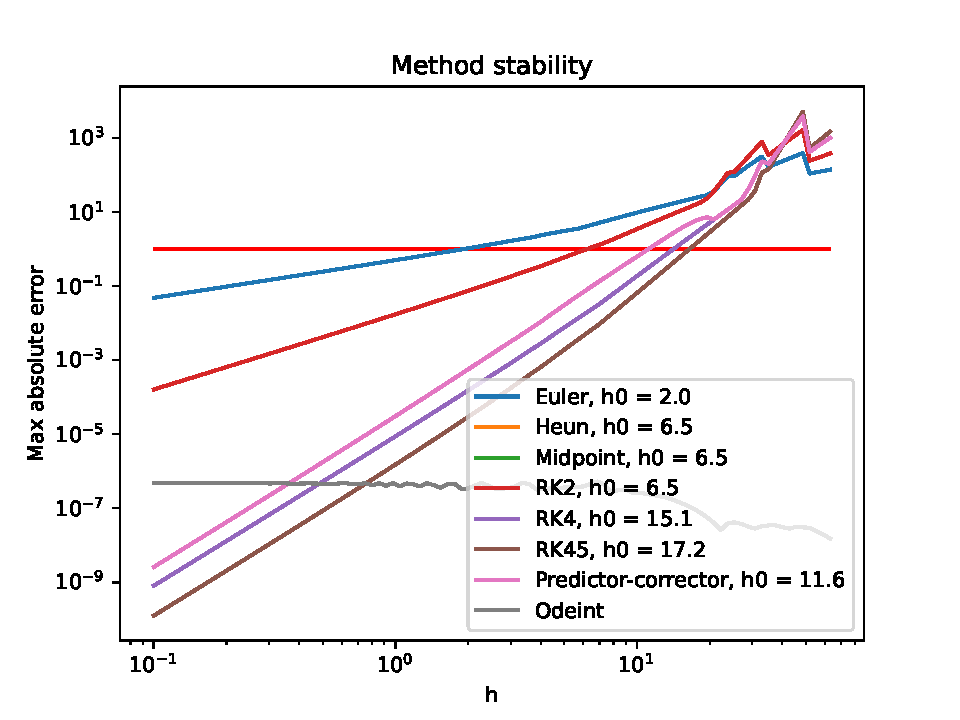
\includegraphics[width=\linewidth]{graphs/stability.pdf}
  \caption{Stability of methods, $error(h_0)=1$} \label{fig:d}
  \end{subfigure} 
  \caption{Analysis of methods} \label{fig:1}
\end{figure}

All the analysis done up to this point looked at points near the initial value, $t << 1$, but here we will look at the opposite limit, $t >> 1$. Doing so will allow us to examine the stability of each method. Figure 2d shows how error increases with step size, where the exact relations between error and $h$ are already known from Figure 2a. What we are interested in are points ($h_0$) where the error surpasses a certain threshold, in our case $1$ (red horizontal line). From the implemented versions the best performing is RK45, where $h_0 = 17.2$ at $t_{max} = 100$. The overall best performing is Odeint which never broke the threshold. All the performance characteristics come from the package ODEPACK written in Fortran which is used in the method {\sc scipy.integrate.odeint}. The method RKF was not analyzed as the step size is not constant.

\begin{figure}[hbtp]
  \begin{center}
  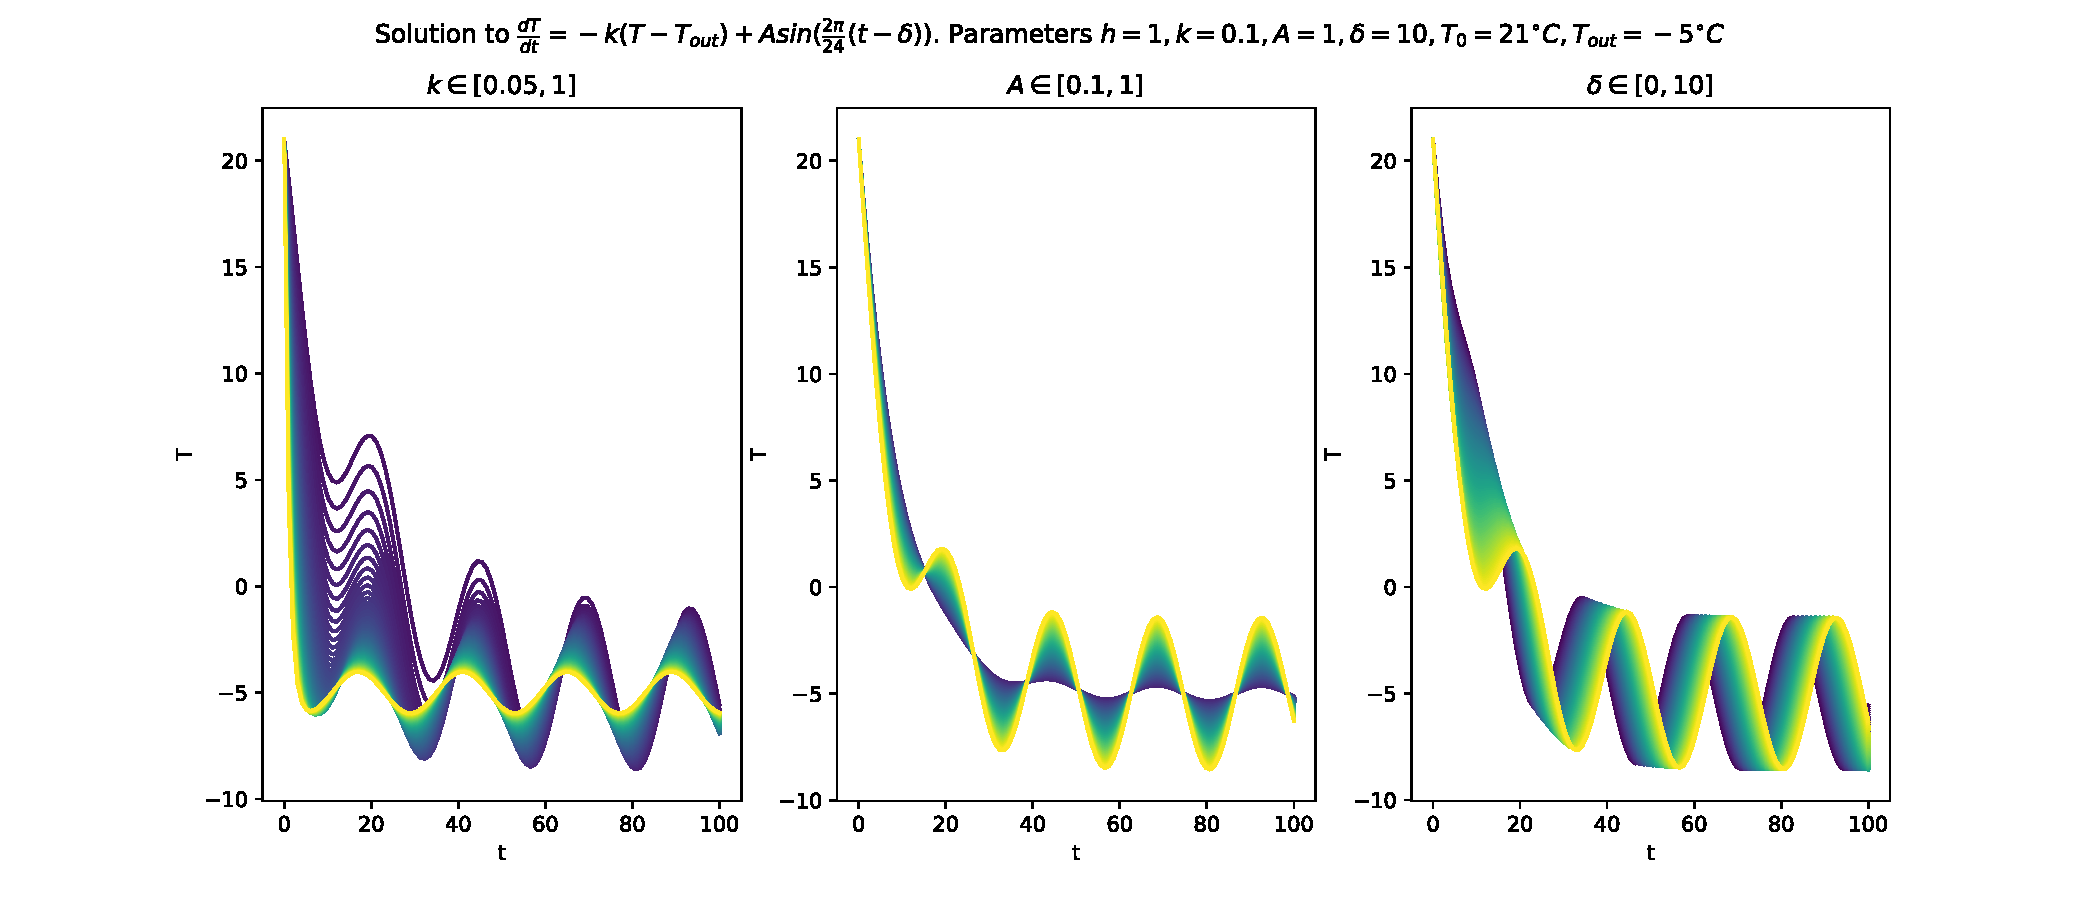
\includegraphics[width=13cm]{graphs/f2.pdf}
  \end{center}
  \vspace*{-7mm}
  \caption{Parameter analysis of solutions for oscillating temperature cycles}
\end{figure}

Additionally we can analyze a variant of the initial problem that follows this equation:
\begin{equation}
  \frac{dT}{dt} = - k \left( T-T_\mathrm{out} \right) + A\sin\left( {2\pi\over 24}(t-\delta) \right)
\end{equation}
This variant includes periodic heating and cooling, which can be associated with day and night temperature oscillations. Here $A$ represents the intensity of the oscillations and $\delta$ the time when we stopped heating the room. The default values are $k = 0.1, A = 1, \delta = 10$ when not stated otherwise. Figure 3 shows the impact of all three parameters on the solution. Based on those graphs parameter $k$ tells us how fast the room is cooling. With lower values of $k$ (violet color) we also notice a phase shift due to the fact that the room has low thermal conductivity. Changing the parameter $A$ we only change the amplitude of the oscillations around the exponential solution. The change in $\delta$ results in the change of phase in the final solution.

\end{document}

